% Taken from:
% https://github.com/codatmo/Liverpool
\documentclass{standalone}

\usepackage{tikz}
\usetikzlibrary{shapes}
\usetikzlibrary{arrows}
\usetikzlibrary{positioning}
\usetikzlibrary{calc}
\usetikzlibrary{fit}
\begin{document}
    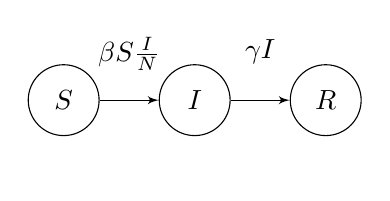
\begin{tikzpicture}[node distance=0.75cm,auto,>=latex',every node/.append style={align=center},int/.style={draw, circle, minimum size=0.9cm}]
        \node [int] (S) {$S$};
        \node [int, right=of S] (I) {$I$};
        \node [int, right=of I] (R) {$R$};

        \path[->, auto=false] (S) edge node {$\beta S \frac{I}{N}$ \\[2.5em]} (I);
        \path[->, auto=false] (I) edge node {$\gamma I$ \\[2.5em]} (R);
    \end{tikzpicture}
\end{document}
